\paragraph{Effect of radius}
For five different radii the maximum dynamic pressure and minimum height above Mars that were encountered on the first pass through the atmosphere were recorded. This is shown in Figure \ref{fig:radius}. For each radius a trajectory for which the spacecraft just reaches the escape velocity (dark blue line, slow trajectory) and a trajectory which decelerates as fast as possible while staying under 3\gls{con:ge} deceleration (light blue line, fast trajectory) are calculated. These two trajectories represent the two boundaries of what could possibly become the final trajectory. To achieve the different trajectories the control (constant angle of attack and changing bank angle) has been adapted. In Figure \ref{fig:radius} it can be seen that there is an approximately quadratic relationship between dynamic pressure and diameter for both limit trajectories. It can also be seen that the fast trajectory has a higher dynamic pressure over the entire range of diameters. This is because the fast trajectory decelerates faster and goes deeper through the atmosphere. The minimal height achieved in the first pass is always $15 \left[km\right]$ for the fast trajectory because in this trajectory the aerocapture and entry phase is terminated at $15 \left[km\right]$ height within the first pass. For the slow trajectory it can be seen that a deeper pass through the atmosphere is needed with a lower diameter aeroshell. The same relation is true for the fast trajectory even though this cannot be seen in this figure. The maximum Mach number encountered is a constant value of Mach 41.7 for changing diameter and also for both limit trajectories.

\begin{figure}[h]
	\centering
	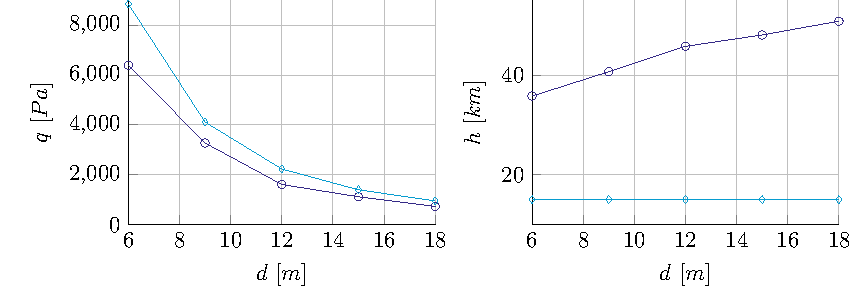
\includegraphics[width=\textwidth]{./Figure/orbit/radius_param2.pdf}
	\caption{Maximum dynamic pressure and Mach number and minimum height for different radii}
	\label{fig:radius}
\end{figure}

Apart from this results it should be noted that there is a lower limit to the diameter of the \gls{cia} imposed by the side heat flux into the capsule. For a large diameter the capsule is in the wake of the \gls{cia} and the side heat flux can thus be neglected. For a smaller diameter aeroshell eventually a backshell will be needed to protect the capsule. This will induce an unacceptable amount of mass.

\paragraph{Effect of lift-to-drag ratio}
During the aerocapture a high lift allows the spacecraft to pass higher through the atmosphere while still having control over the vehicle, thus having the ability to stay in the atmosphere longer. The drag should also be high during the aerocapture in order to have the ability to lose enough energy.

During the entry \& descent phase a high lift gives better control over the final landing position. The deceleration during this phase is however quickly too high, so a lower drag is required.

As the aerocapture and entry \& descent phases both have to deal with the same aerodynamic properties a compromise has to be made on the drag, however the lift should be high for both phases.

\paragraph{Entry corridor}
The entry corridor is the fictional box where the entry vehicle should pass through to go into orbit. Too low and the acceleration limit or the heat limit is breached, too high and the entry vehicle will skip on the atmosphere and never return. This corridor is dependent on different design parameters, the most important are the aerodynamic coefficients, entry velocity and control system.

\begin{figure}[h]
	\centering
	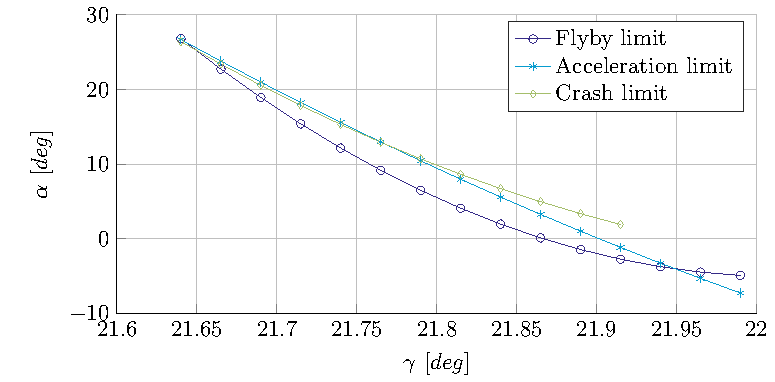
\includegraphics[width=\textwidth]{./Figure/orbit/alpha_gamma.pdf}
	\caption[The entry corridor for different angles of attack and flight path angles]{The entry corridor for different angles of attack and flight path angles. This figure is computed with the final aerodynamic shape, the aerocapture \gls{sym:mu}-profile, and an entry velocity (\gls{sym:V}) of $7000 \left[m\cdot s^{-1}\right]$}
	\label{fig:alpha_gamma}
\end{figure}

From a point in the middle of the entry corridor, as shown in Figure \ref{fig:alpha_gamma}, the initial flight path angle (\gls{sym:gamma}), the angle of attack (\gls{sym:alpha}) and the bank angle (\gls{sym:mu}) have been changed to the utmost points where an orbit was still achieved. The effects of these changes separately are presented below.

\paragraph{Effect of initial flight path angle}
As can be seen in Figure \ref{fig:effectgamma} the range of initial flight path angle for which an orbit is achieved is very limited. This means \gls{sym:gamma} has a big effect on the trajectory. For this small change in flight path angle the maximum dynamic pressure (\gls{sym:q}) increases by approximately $400$ $\left[Pa\right]$. It can also be seen the minimum height (\gls{sym:h}) decreases by more than two kilometres. The maximum Mach number (\gls{sym:M}) does not change for changing initial flight path angle.

\begin{figure}[h]
	\centering
	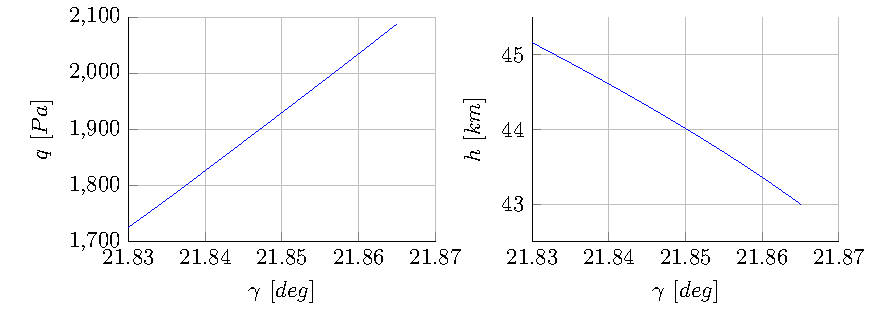
\includegraphics[width=\textwidth]{./Figure/orbit/effectgamma2.pdf}
	\caption[Effect on dynamic pressure, height and Mach number of different flight path angles]{Effect on dynamic pressure, height and Mach number of different flight path angles at $\gls{sym:alpha}=15$ $\left[deg\right]$ and $\gls{sym:mu}=30$ $\left[deg\right]$}
	\label{fig:effectgamma}
\end{figure}

\paragraph{Effect of angle of attack}

In Figure \ref{fig:effectalpha} the range of angle of attack for which an orbit is achieved is shown. It can be observed that this window is five degrees wide. This means that the effect of \gls{sym:alpha} on the trajectory is significantly smaller than the effect of the flight path angle. However for this bigger change in angle still a big change both dynamic pressure and height is encountered. The maximum dynamic pressure increases by approximately $300 \left[Pa\right]$. It can also be seen the minimum height decreases by almost two kilometres. The maximum Mach number does not change for changing angle of attack.

\begin{figure}[h]
	\centering
	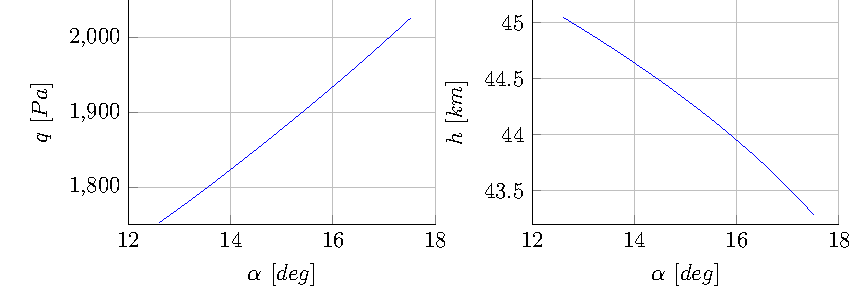
\includegraphics[width=\textwidth]{./Figure/orbit/effectalpha2.pdf}
	\caption[Effect on dynamic pressure, height and Mach number of different angles of attack]{Effect on dynamic pressure, height and Mach number of different angles of attack at $\gls{sym:gamma}=21.845$ $\left[deg\right]$ and $\gls{sym:mu}=30$ $\left[deg\right]$}
	\label{fig:effectalpha}
\end{figure}

\paragraph{Effect of bank angle}

As can be seen in Figure \ref{fig:effectmu} the range for which an orbit is achieved changing only bank angle is almost $60 \left[deg\right]$. This means \gls{sym:mu} has to be changed a lot, compared to \gls{sym:gamma} and \gls{sym:alpha}, to have an effect on the orbit. This change in bank angle does not have a big effect on the maximum dynamic pressure and the height. This indicates that the change in trajectory caused by a change in bank angle is much more subtle. The maximum Mach number does not change for changing bank angle.

\begin{figure}[h]
	\centering
	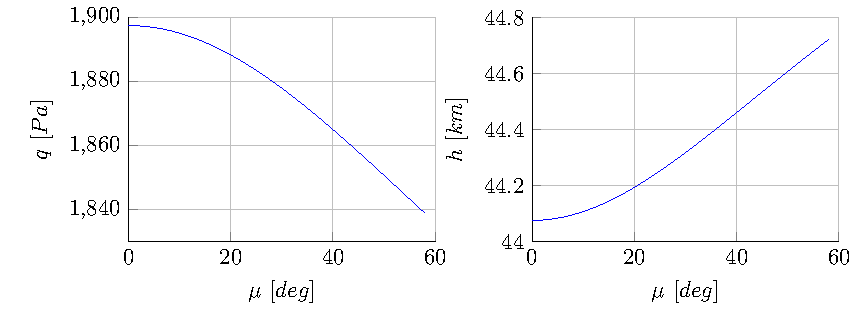
\includegraphics[width=\textwidth]{./Figure/orbit/effectmu2.pdf}
	\caption[Effect on dynamic pressure, height and Mach number of different bank angles]{Effect on dynamic pressure, height and Mach number of different bank angles at $\gls{sym:alpha}=15$ $\left[deg\right]$ and $\gls{sym:gamma}=21.845$ $\left[deg\right]$}
	\label{fig:effectmu}
\end{figure}